\section{WebGL}

\subsection{Pipeline}
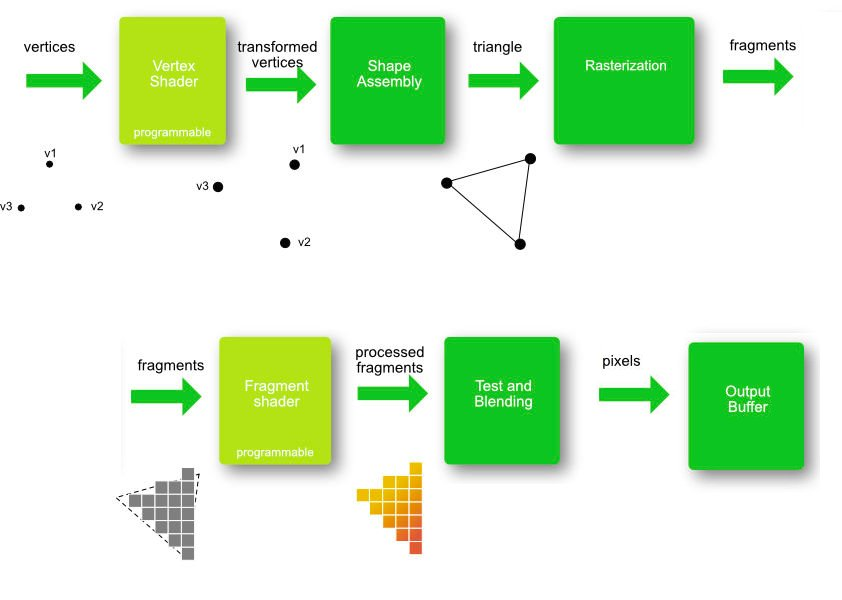
\includegraphics[width=0.9\textwidth]{images/graphicPipeline.jpg}

WebGL does
\begin{itemize}
    \item calculate the projection of your 3d-vertices onto a flat 2d plane
    \item calculate how faces occude each other
    \item rasterize all visible faces
\end{itemize}

WebGL does not 
\begin{itemize}
    \item provide a render loop
\end{itemize}

\subsection{Slang}

First, we need to explain some jargon. 
\begin{itemize}
    \item \emph{context}: a set of slots that users can access to manipulate data. Most important slot: \inlinecode{gl.ARRAY_BUFFER}
    
    \item \emph{buffer}: a object of data that can be provided to a shader.

    \item \emph{The vertrex shader} is called once for every vertex. It does some transformation on the vertex to add perspective and then stores the result in \inlinecode{gl_Position}. 
    Note that these shaders cannot add vertices, they can only modify them. A good usage example is motion-distortion (making objects passing by look distorted) or water rippeling.
    
    \item \emph{The fragment shader} is called once for every pixel on every shape. It determines the pixel's color (\inlinecode{gl_FragColor}) by
    \begin{itemize}
        \item which pixel of a texture belongs here, 
        \item applying lighting and shadows
    \end{itemize} 
\end{itemize}



\subsection{Buffers: webGL's abstract data-structures}

Passing data in to webGL: 
\begin{itemize}
    \item Generate a buffer and get its id: \inlinecode{let id: number = gl.createBuffer();}
    \item The \inlinecode{ARRAY_BUFFER} is a place where a buffers data may be modified. \inlinecode{gl.bindBuffer(gl.ARRAY_BUFFER, id);}
    \item Put in actual data. \inlinecode{gl.bufferData(gl.ARRAY_BUFFER, [1.2, 3.2, 4.0], gl.STATIC_DRAW);}
\end{itemize}


\subsection{Compiling a shader program}

We'll use these two shaders as an example: 

\begin{lstlisting}[language=c, caption=vertex-shader]
attribute vec4 aVertexPosition;

uniform mat4 uModelViewMatrix;
uniform mat4 uProjectionMatrix;

void main() {
    gl_Position = uProjectionMatrix * uModelViewMatrix * aVertexPosition;
}
\end{lstlisting}

\begin{lstlisting}[language=c, caption=pixel-shader]
    void main() {
      gl_FragColor = vec4(1.0, 1.0, 1.0, 1.0);
    }
\end{lstlisting}

\begin{itemize}
    \item Datatypes are \inlinecode{vec3, vec4, mat3, mat4, }
    \item \inlinecode{const} – The declaration is of a compile time constant.
    \item \inlinecode{attribute} – Global variables that may change per vertex, that are passed from the OpenGL application to vertex shaders. This qualifier can only be used in vertex shaders. For the shader this is a read-only variable.
    \item \inlinecode{uniform} – Global variables that may change per primitive [...], that are passed from the OpenGL application to the shaders. This qualifier can be used in both vertex and fragment shaders. For the shaders this is a read-only variable.
    \item \inlinecode{varying} – used for interpolated data between a vertex shader and a fragment shader. Available for writing in the vertex shader, and read-only in a fragment shader.
\end{itemize}

This is how to compile those shaders and provide them to webGL.

\begin{lstlisting}[language=java]

function compileShader(gl, typeBit, shaderSource) {
    const shader = gl.createShader(typeBit);
    gl.shaderSource(shader, shaderSource);
    gl.compileShader(shader);
    if(!gl.getShaderParameter(shader, gl.COMPILE_STATUS)) {
        alert('An error occurred compiling the shaders: ' + gl.getShaderInfoLog(shader));
        gl.deleteShader(shader);
        return null;
    }
    return shader;
}

function initShaderProgram(gl, vertexShaderSource, fragmentShaderSource) {
    const vertexShader = compileShader(gl, gl.VERTEX_SHADER, vertexShaderSource);
    const fragmentShader = compileShader(gl, gl.FRAGMENT_SHADER, fragmentShaderSource);
    const shaderProgram = gl.createProgram();
    gl.attachShader(shaderProgram, vertexShader);
    gl.attachShader(shaderProgram, fragmentShader);
    gl.linkProgram(shaderProgram);
    if(!gl.getProgramParameter(shaderProgram, gl.LINK_STATUS)) {
        alert('Unable to initialize the shader program: ' + gl.getProgramInfoLog(shaderProgram));
        return null;
    }
    return shaderProgram;
}
\end{lstlisting}

\subsection{Setting up webGL}

Finally, we start webGL with the compiled program.
\begin{lstlisting}[language=java]

function setupScene(gl, program) {
    gl.clearColor(0.0, 0.0, 0.0, 1.0);
    gl.clearDepth(1.0);
    gl.enable(gl.DEPTH_TEST);
    gl.depthFunc(gl.LEQUAL);
    gl.clear(gl.COLOR_BUFFER_BIT | gl.DEPTH_BUFFER_BIT);
    gl.useProgram(program);
}

const canvas = document.getElementById("glCanvas");
const gl = canvas.getContext("webgl");
const shaderProgram = initShaderProgram(gl, vertexShaderSource, fragmentShaderSource);
setupScene(context, shaderProgram);
\end{lstlisting}

\subsection{Putting data into a uniform}

Uniforms will remain the same for all vertices. 

\begin{lstlisting}[language=java]
const modelViewMatrix = mat4.create();
mat4.translate(modelViewMatrix, modelViewMatrix, [-0.0, 0.0, -6.0]);

const viewMatrixPosition = gl.getUniformLocation(shaderProgram, 'uModelViewMatrix');

gl.uniformMatrix4fv(viewMatrixPosition, false, modelViewMatrix);
\end{lstlisting}

\subsection{Putting data from buffer into a vertex'es attribute)}

Attributes may vary between vertices (though, like uniforms, they are still read-only for the shader). Because they are not globally the same, contrary to uniforms they must be set via buffers. 

\begin{itemize}
    \item Get the location of the target-attribute. \inlinecode{let position = gl.getAttribLocation(program, "aVertexPosition")}
    \item Make the target-attribute editable (one-time only?) \inlinecode{gl.enableVertexAttribArray(position);}
    \item Dock the data-containing buffer to the context. \inlinecode{gl.bindBuffer(gl.ARRAY_BUFFER, positionDataBuffer)}
    \item Retrieve the data from the buffer. \inlinecode{gl.vertexAttribPointer(position, numComponents, typeOfData, normalizeFlag, strideToNextPieceOfData, offsetIntoBuffer)} 
        \begin{itemize}
            \item Number of components is always 1 to 4. 
            \item If you are using 1 buffer per type of data then both stride and offset can always be 0. 0 for stride means "use a stride that matches the type and size". 0 for offset means start at the beginning of the buffer. Setting them to values other than 0 is more complicated and though it has some benefits in terms of performance it's not worth the complication unless you are trying to push WebGL to its absolute limits.
        \end{itemize}
\end{itemize}



